\documentclass[11pt]{easymemo}

\SectionNumber
%\BlackAndWhite

\begin{document}

\MakeTitle{2026.10.18}{MultiPieの基底の生成法の改良 (考察中)}{明大理工 楠瀬博明}


\section{前提}
\begin{itemize}
\item ITAの標準セッティングのみ使用。
\item 対称操作とWyckoff位置の順序はITAと同一。
\item 対称操作と一般点のWyckoff位置の順序は一対一対応している。
\item 結晶点群と空間群の対称操作の順序は部分並進を除くと一致する。
\end{itemize}

\section{ルートクラスター}

\subsection{サイトおよびボンドルートクラスター}

この節ではデカルト座標を用いる。
$O_{\rm h}$および$D_{\rm 6h}$の一般点を含み、なるべく球形に近いクラスターを構成することを考える。
まず、$D_{\rm 6h}$の対称操作を$g_i$ ($i=1,\cdots,24$)とする。
主軸を$z':[111]$、副軸を$x':[\bar{1}10]$, $y':[\bar{1}\bar{1}2]$に変換し
\begin{align}
g_i^{[111]}=R_cg_iR_c^{-1},
\quad
R_c = \begin{pmatrix}
-\frac{1}{\sqrt{2}} & -\frac{1}{\sqrt{6}} & \frac{1}{\sqrt{3}} \\
\frac{1}{\sqrt{2}} & -\frac{1}{\sqrt{6}} & \frac{1}{\sqrt{3}} \\
0 & \frac{2}{\sqrt{6}} & \frac{1}{\sqrt{3}}
\end{pmatrix}
\end{align}
代表点$\bm{r}_0=[x,y,z]$に変換後の対称操作を行って$\bm{r}_i=g_i^{[111]}\bm{r}_0$を定義する。
次に、得られた点群$\bm{r}_i$に$x,y,z$軸周りの$\pi$回転$R_x,R_y,R_z$を行って得られた点群を加える。
これらを$\bm{r}_{i+24}=R_x\bm{r}_i$, $\bm{r}_{i+48}=R_y\bm{r}_i$, $\bm{r}_{i+72}=R_z\bm{r}_i$とする。
以上で、$24\times 4=96$個の点群が得られる。
このクラスターをルートクラスターと呼ぶことにする。
なお、主軸を$[1\bar{1}\bar{1}]$, $[\bar{1}1\bar{1}]$, $[\bar{1}\bar{1}1]$に取った対称操作を$g_i^{[1\bar{1}\bar{1}]}=R_xg_i^{[111]}R_x$, $g_i^{[\bar{1}1\bar{1}]}=R_yg_i^{[111]}R_y$, $g_i^{[\bar{1}\bar{1}1]}=R_zg_i^{[111]}R_z$とすると、$\bm{r}_{i+24}=g_i^{[1\bar{1}\bar{1}]}(R_x\bm{r}_0)$, $\bm{r}_{i+48}=g_i^{[\bar{1}1\bar{1}]}(R_y\bm{r}_0)$, $\bm{r}_{i+72}=g_i^{[\bar{1}\bar{1}1]}(R_z\bm{r}_0)$の関係がある。

ルートクラスターの点群は、$O_{\rm h}$の対称操作$\bar{g}_i$ ($i=1,\cdots,48$)および$[\bar{1}\bar{1}2]$面に関する鏡映$M$を用いて
\begin{align}
\bar{\bm{r}}_i=\bar{g}_i\bm{r}_0,
\quad
\bar{\bm{r}}_{i+48}=\bar{g}_i(M\bm{r}_0),
\quad
M=\begin{pmatrix}
\frac{2}{3} & -\frac{1}{3} & \frac{2}{3} \\ -\frac{1}{3} & \frac{2}{3} & \frac{2}{3} \\ \frac{2}{3} & \frac{2}{3} & -\frac{1}{3}
\end{pmatrix}
\end{align}
のように得られる\footnote{鏡映操作$M$は$\bar{g}_i$を$O_{\rm h}$に含まれない対称操作に変えてしまうので、$\bar{\bm{r}}_{i+48}=M\bar{\bm{r}}_i$は成り立たないことに注意する。}。
$\bm{r}_j$と$\bar{\bm{r}}_j$ ($j=1,\cdots,96$)の並び順は異なるが一対一対応がある。
ルートクラスターの点と対称操作の区分を図\ref{fig:vc}および\ref{fig:vc_no}に示す。
構成方法から分かるようにルートクラスターは空間反転対称性がある。

具体的な値が必要なときは$\bm{r}_0=[5,\sqrt{3},2]$を用いる\footnote{sympy計算が複雑にならないよう規格化しない。空間群のWyckoff位置を例示するときは$[x,y,z]$に範囲制限があることを考慮して、$\bm{r}_0/s$を用いる。スケール因子$s$の典型値は$s=5$。}。
また、ボンドのクラスターを作成するには$\bm{r}_j\to\bm{v}_j@\bm{c}_j$ ($\bm{v}_j$は$\bm{r}_j$の内容を大文字に置き換えたもの、$\bm{c}_j=\bm{r}_j$)とすればよい。
具体的な値として$\bm{v}_0=[\sqrt{3},5,2]$を用いる\footnote{ボンドクラスター基底の生成に用いるが、ベクトル基底とボンドの内積が偶然消えないよう、$\bm{v}_0$は$\bm{r}_0$と平行でも垂直でもないように取る必要がある。また、規格化しない理由は$\bm{r}_0$と同じ。}。

\begin{figure}[t]
\caption{ルートクラスター。$D_{\rm 6h}$の主軸ごとに色分けした。}
\label{fig:vc}
\begin{center}
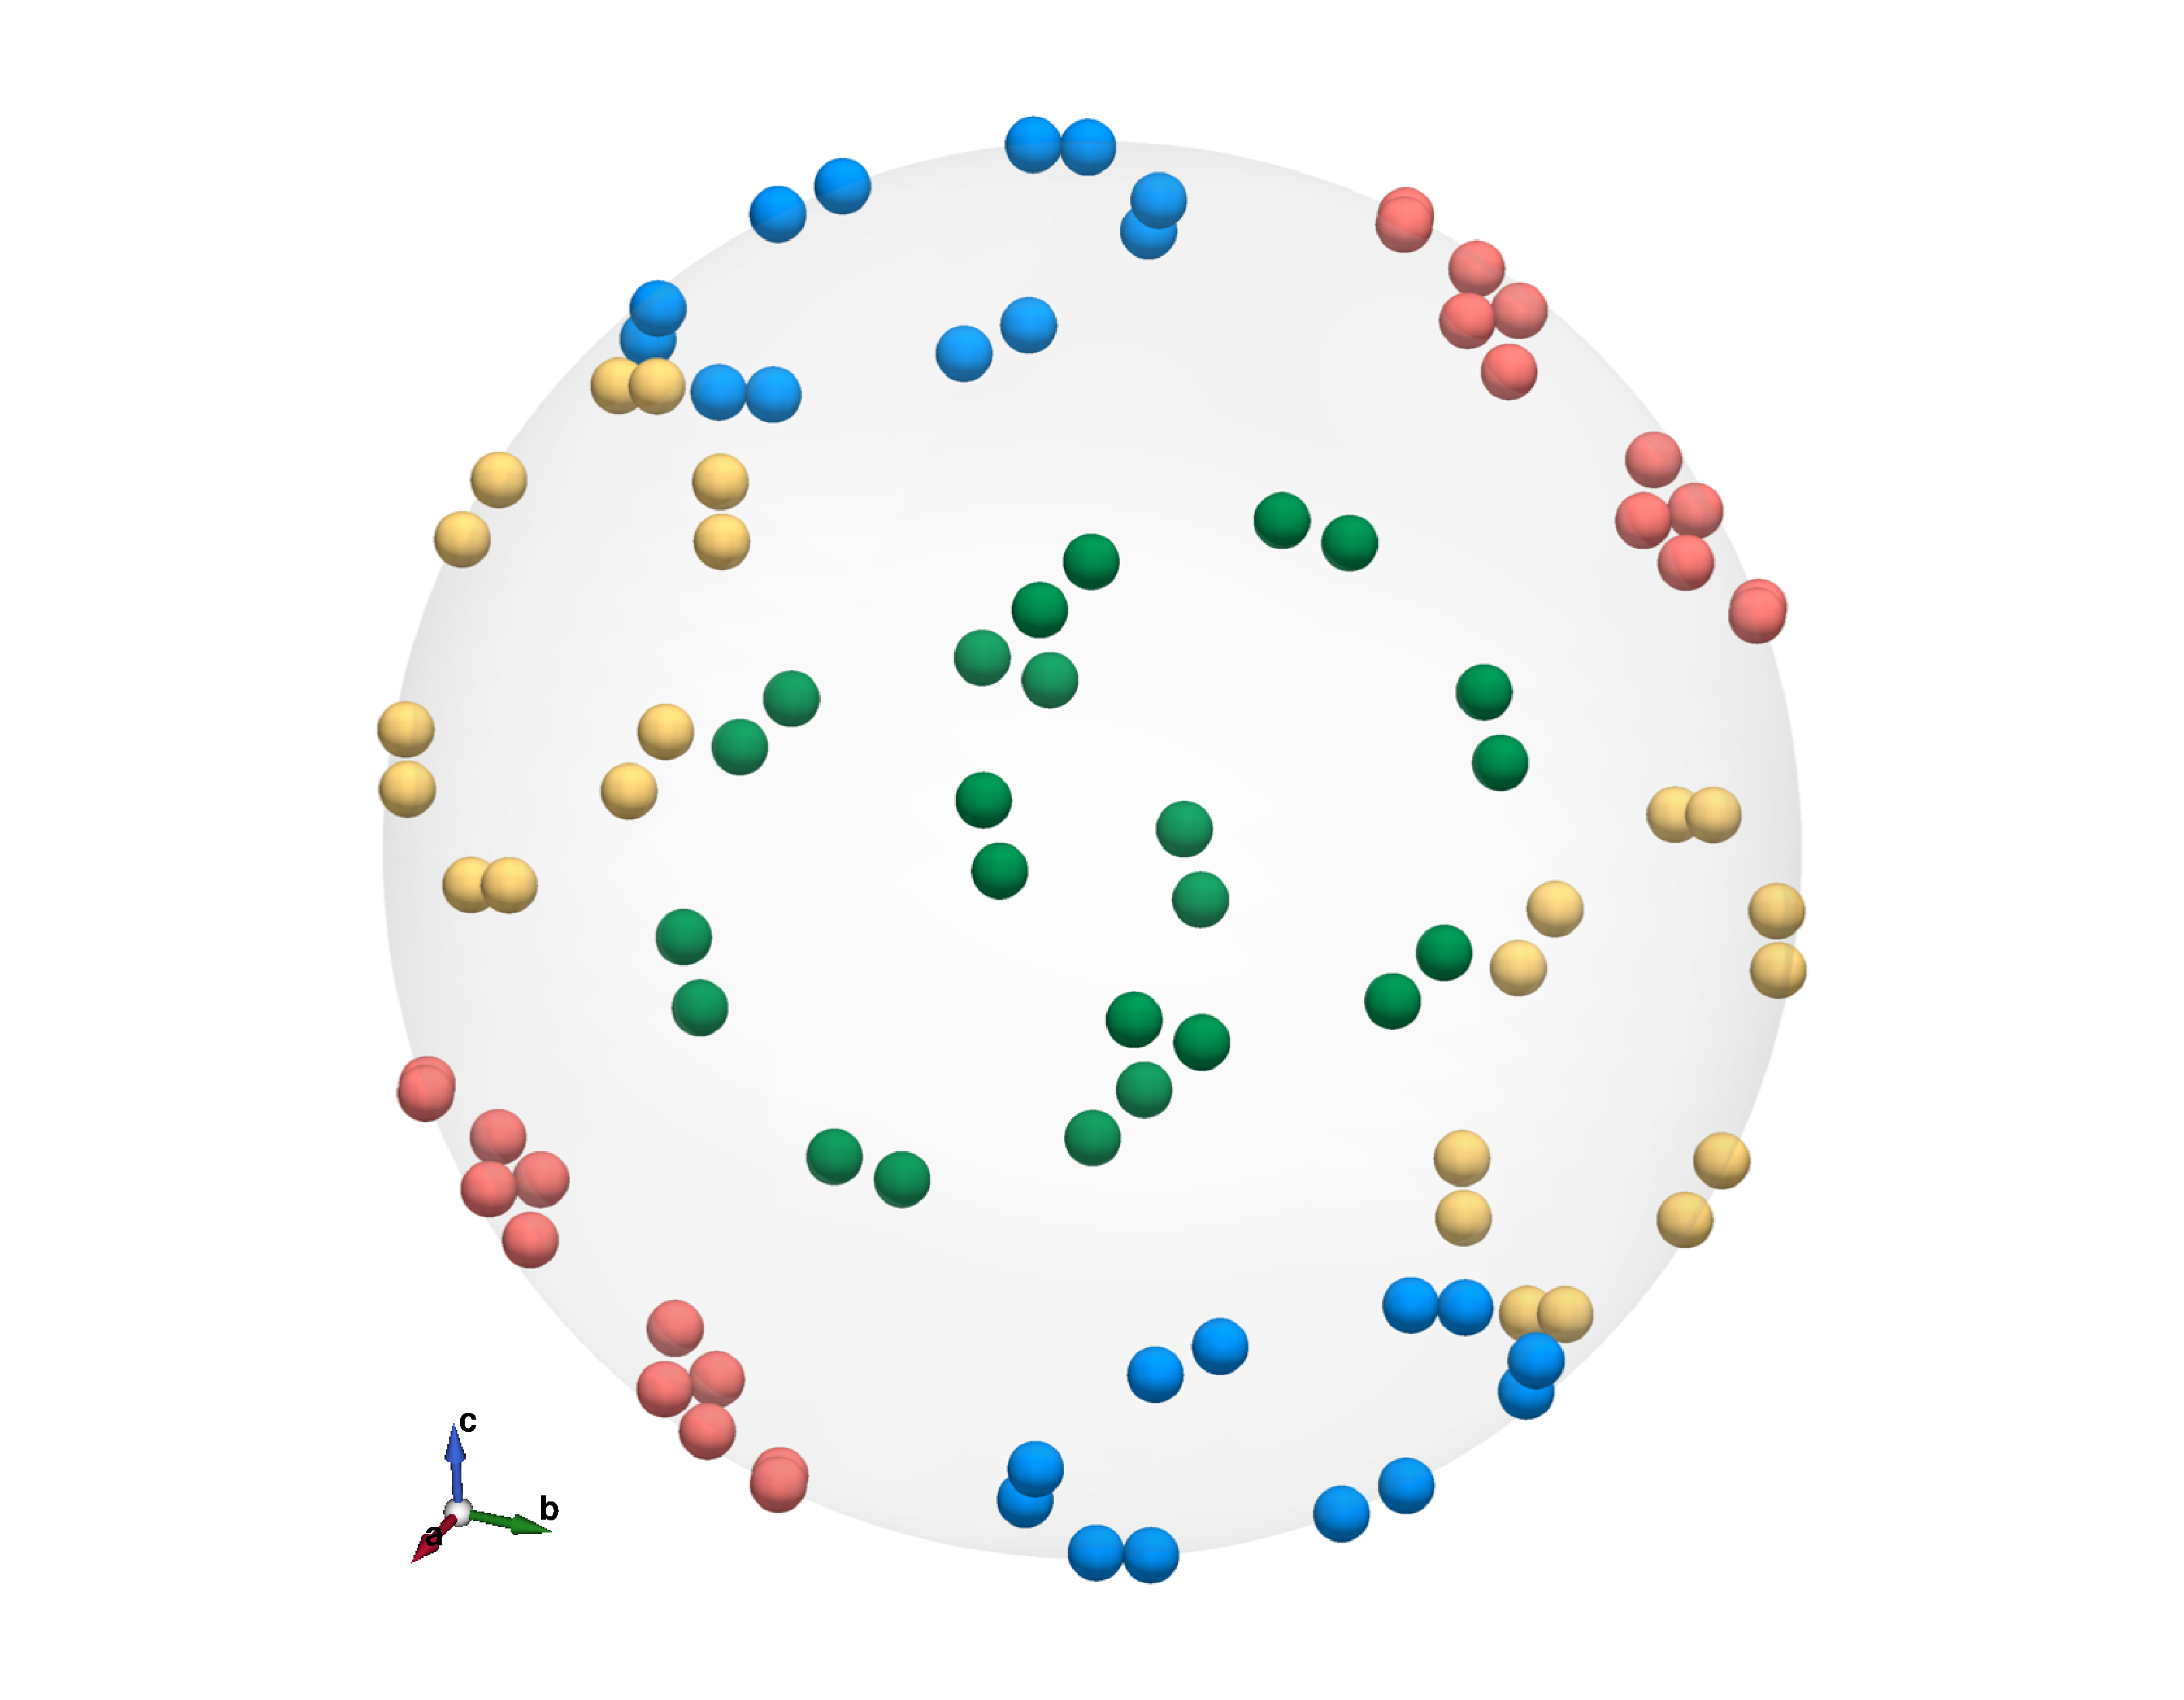
\includegraphics[width=6cm]{vc.eps}
\end{center}
\end{figure}
\begin{figure}[t]
\caption{ルートクラスターの対称操作区分。}
\label{fig:vc_no}
\begin{center}
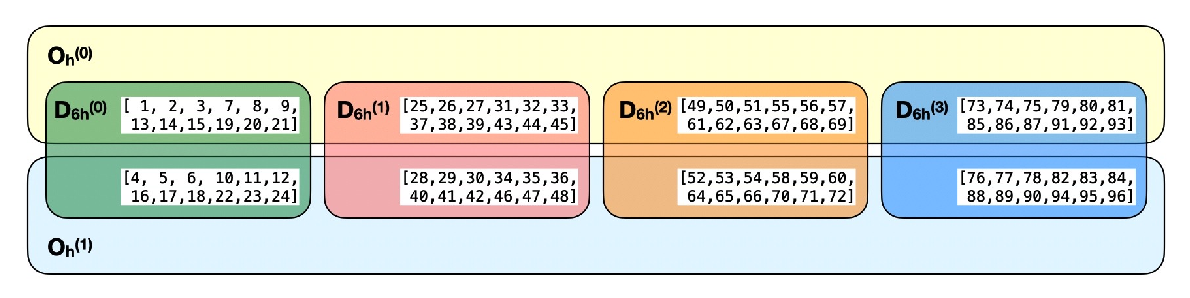
\includegraphics[width=15cm]{vc_no.eps}
\end{center}
\end{figure}

\subsection{ルートクラスター基底}

サイトやボンドのクラスター基底を構成するために必要なルートクラスター上の多極子基底は、デカルト座標系の方域表示($m\geqq 0$は$C$, $m<0$は$S$を意味すると約束する)で\footnote{ベクトル球面調和関数の内部自由度は極性ベクトルで$xyz$の直交基底を用いる。}
\begin{align}
\vec{Q}_{lm}=[Q_{lm}(\bm{r}_j)],
\quad
\vec{Q}_{lm}^{(v,\pm)}=[\bm{Q}_{lm}^{(1,\pm1)}(\bm{r}_j)],
\quad
\vec{G}_{lm}^{(v,0)}=[\bm{G}_{lm}^{(1,0)}(\bm{r}_j)]
\end{align}
である。
ここで、偶(奇)パリティの基底は$l=偶数(奇数)$の$\vec{Q}_{lm}$, $\vec{Q}_{lm}^{(v,\pm)}$と$l=奇数(偶数)$の$\vec{G}_{lm}^{(v,0)}$である。
また、ボンドベクトルは$\vec{b}=[\bm{v}_j@\bm{c}_j]$により定義される。
ボンドベクトルは、ルートクラスターの各点を生成する対称操作によって生成されるから、空間反転に関して偶である。
したがって、$\vec{Q}_{lm}^{(v,\pm)}$や$\vec{G}_{lm}^{(v,0)}$と$\vec{b}$との内積は多極子基底のタイプを変えない。
そこで
\begin{align}
\vec{Q}_{lm}^{(\pm)}=[\bm{v}_j\cdot\bm{Q}_{lm}^{(1,\pm1)}(\bm{r}_j)],
\quad
\vec{G}_{lm}^{(0)}=[\bm{v}_j\cdot\bm{G}_{lm}^{(1,0)}(\bm{r}_j)]
\end{align}
を導入しておく。
$l=9$ ($100$また$300$基底)まで生成しておけば実用上十分である。

$\vec{Q}_{lm}$, $\{\vec{Q}_{lm}^{(\pm)},\vec{G}_{lm}^{(0)}\}$は$96$個が独立、$\{\vec{Q}_{lm}^{(v,\pm)},\vec{G}_{lm}^{(v,0)}\}$は$96\times 3=288$個が独立である。
正規直交化するときは、$\bm{r}_0$や$\bm{v}_0$に代表値を代入し、ランクの低い順かつ同ランクでは$\vec{Q}_{lm}^{(-)}$, $\vec{G}_{lm}^{(0)}$, $\vec{Q}_{lm}^{(+)}$の順で行う。
$v$の上付きの場合も同様。

$D_{\rm 6h}^{(0)}$および$O_{\rm h}^{(0)}$の構成(対称操作順)
\begin{codebox}
d6h (24g) =
[ 1, 2, 3, 4, 5, 6, 7, 8, 9,10,11,12,13,14,15,16,17,18,19,20,21,22,23,24]
oh (48f) =
[ 1,92,67,45, 2,43,93,68, 3,69,44,91,85, 8,62,39,86,37, 9,63,87,61,38, 7,
 13,80,55,33,14,31,81,56,15,57,32,79,73,20,50,27,74,25,21,51,75,49,26,19]
\end{codebox}

\textcolor{red}{
$O_{\rm h}$および$D_{\rm 6h}$の$\vec{Q}_{lm}$, $\{\vec{Q}_{lm}^{(\pm)},\vec{G}_{lm}^{(0)}\}$基底(48,24)個を正規直交化して生成。点群調和関数で。
空間群についてもマッピング表を作成。$D_{\rm 6h}^i$と$O_{\rm h}^i$の14個の空間群について、基底生成。
オプションで、内部rank 3までの多極子調和関数も。
}



\section{ルートクラスターと$O_{\rm h}$, $D_{\rm 6h}$の関係}

ルートクラスターと$O_{\rm h}$, $D_{\rm 6h}$の関係を考える。
ルートクラスターのうち、図\ref{fig:vc_no}の$O_{\rm h}^{(0)}$と$D_{\rm 6h}^{(0)}$のグループを用いる。
$D_{\rm 6h}$の基底を生成するときは、$[111]$を$z$軸に取り直す。
$O_{\rm h}$と$D_{\rm 6h}$の基底を比較するときは、共通の12点を対称操作の対応関係を用いて行う。


\section{部分群との関係}

結晶点群は回転群の部分群であり、各結晶点群間にも部分群の関係がある。
親群(p)の対称操作と部分群(c)の対称操作(1から)の関係をリスト\texttt{coset[n][j]}を用いて
\begin{align}
&
\hat{g}_{\rm p}[{\rm coset}[0][i-1]]=\hat{R}\hat{g}_{\rm c}[i]\hat{R}^{-1},
\quad
(i=1,2,\cdots)
\cr&
\hat{g}_{\rm p}[{\rm coset}[n][i-1]]=\hat{g}_{\rm parent}^{(n)}\hat{g}_{\rm p}[{\rm coset}[0][i-1]]
\quad
(n=1,2,\cdots)
\end{align}
と表す。
ここで$\hat{g}_{\rm p}^{(n)}$は、親群の部分群に含まれない対称操作(の代表)を表す。
空間群の場合も$\hat{R}$が$4\times4$になること以外は同様である。
$\hat{R}$は主軸変換の行列であり、単位行列になるべく近く、また空間群では原点移動が小さくなるように選ばれている。
結晶点群について親群と部分群の関係を表\ref{tbl:1}に示す。
必要な主軸変換行列は分率座標系で
\begin{align}
&
\hat{R}_c = \begin{pmatrix}
-\frac{1}{\sqrt{2}} & -\frac{1}{\sqrt{6}} & \frac{1}{\sqrt{3}} \\
\frac{1}{\sqrt{2}} & -\frac{1}{\sqrt{6}} & \frac{1}{\sqrt{3}} \\
0 & \frac{2}{\sqrt{6}} & \frac{1}{\sqrt{3}}
\end{pmatrix},
\quad
\hat{R}_{c1} = \begin{pmatrix} -\frac{1}{\sqrt{6}} & \frac{1}{\sqrt{2}} & \frac{1}{\sqrt{3}} \\
-\frac{1}{\sqrt{6}} & -\frac{1}{\sqrt{2}} & \frac{1}{\sqrt{3}} \\
\frac{2}{\sqrt{6}} & 0 & \frac{1}{\sqrt{3}}
\end{pmatrix},
\quad
\hat{R}_t = \begin{pmatrix} \frac{1}{\sqrt{2}} & \frac{1}{\sqrt{2}} & 0 \\
-\frac{1}{\sqrt{2}} & \frac{1}{\sqrt{2}} & 0 \\
0 & 0 & 1
\end{pmatrix}
\cr&
\hat{R}_x = \begin{pmatrix} 1 & 0 & 0 \\ 0 & 0 & 1 \\ 0 & -1 & 0 \end{pmatrix},
\quad
\hat{R}_y = \begin{pmatrix} 0 & 0 & -1 \\ 0 & 1 & 0 \\ 1 & 0 & 0 \end{pmatrix},
\quad
\hat{R}_z = \begin{pmatrix} 0 & 1 & 0 \\ -1 & 0 & 0 \\ 0 & 0 & 1 \end{pmatrix}
\end{align}
また、デカルト座標系と分率座標系の変換行列は
\begin{align}
T = \begin{pmatrix} 1 & -\frac{1}{2} & 0 \\ 0 & \frac{\sqrt{3}}{2} & 0 \\ 0 & 0 & 1 \end{pmatrix}
\end{align}
である。
すべての結晶点群の一般点はルートクラスターに含まれ、特殊点は一般点を平均化することにより得られる。

\begin{table}[t]
\caption{親群と部分群の関係。}
\label{tbl:1}
\begin{center}
\scriptsize
\begin{tabular}{ccc} \hline\hline
child & parent & c-axis -> p-axis ($\hat{R}$) \\ \hline
C$_1$ & C$_{\rm i}$ & \\
   & C$_2$ & \\
   & C$_{\rm s}$ & \\
   & C$_3$ & \\ \hline
C$_{\rm i}$ & C$_{\rm 2h}$ & \\
   & C$_{\rm 3i}$ & \\ \hline\hline
C$_2$ & C$_{\rm 2h}$ & \\
   & D$_2$ & [010]->[001]:$R_x$ \\
   & C$_{\rm 2v}$ & [010]->[001]:$R_x$ \\
   & C$_4$ & [010]->[001]:$R_x$ \\
   & S$_4$ & [010]->[001]:$R_x$ \\
   & D$_3$ & [010]->[100]:$T^{-1}R_z$ \\
   & D$_3(1)$ & [010]->[120]:$T^{-1}$ \\
   & C$_6$ & [010]->[001]:$T^{-1}R_x$ \\ \hline
C$_{\rm s}$ & C$_{\rm 2h}$ & \\
   & C$_{\rm 2v}$ & \\
   & C$_{\rm 3v}$ & [010]->[100]:$T^{-1}R_z$ \\
   & C$_{\rm 3v}(1)$ & [010]->[120]:$T^{-1}$ \\
   & C$_{\rm 3h}$ & [010]->[001]:$T^{-1}R_x$ \\ \hline
C$_{\rm 2h}$ & D$_{\rm 2h}$ & \\
   & C$_{\rm 4h}$ & [010]->[001]:$R_x$ \\
   & C$_{\rm 6h}$ & [010]->[001]:$T^{-1}R_x$ \\
   & D$_{\rm 3d}$ & [010]->[100]:$T^{-1}R_z$ \\
   & D$_{\rm 3d}(1)$ & [010]->[120]:$T^{-1}$ \\ \hline\hline
D$_2$ & D$_{\rm 2h}$ & \\
   & D$_4$ & \\
   & D$_{\rm 2d}$ & \\
   & D$_{\rm 2d}(1)$ & [100]->[110]:$R_t$ \\
   & D$_6$ & $T^{-1}$ \\
   & T & \\ \hline
C$_{\rm 2v}$ & D$_{\rm 2h}$ & \\
    & C$_{\rm 4v}$ & \\
    & D$_{\rm 2d}$ & [100]->[110]:$R_t$ \\
    & D$_{\rm 2d}(1)$ & \\
    & C$_{\rm 6v}$ & $T^{-1}$ \\
    & D$_{\rm 3h}$ & [010]->[001]:$T^{-1}R_x$ \\
    & D$_{\rm 3h}(1)$ & [100]->[001]:$T^{-1}R_y$ \\ \hline
D$_{\rm 2h}$ & D$_{\rm 4h}$ & \\
    & D$_{\rm 6h}$ & $T^{-1}$ \\
    & T$_{\rm h}$ & \\ \hline\hline
C$_4$ & C$_{\rm 4h}$ & \\
   & D$_4$ & \\
   & C$_{\rm 4v}$ & \\ \hline
S$_4$ & C$_{\rm 4h}$ & \\
   & D$_{\rm 2d}$ & \\
   & D$_{\rm 2d}(1)$ & \\ \hline
C$_{\rm 4h}$ & D$_{\rm 4h}$ & \\ \hline
D$_4$ & D$_{\rm 4h}$ & \\
   & O & \\ \hline
C$_{\rm 4v}$ & D$_{\rm 4h}$ & \\ \hline
D$_{\rm 2d}$ & D$_{\rm 4h}$ & \\
    & T$_{\rm d}$ & \\ \hline,
D$_{\rm 2d}(1)$ & D$_{\rm 4h}$ & \\
      & T$_{\rm d}$ & [100]->[110]:$R_t$ \\ \hline
D$_{\rm 4h}$ & O$_{\rm h}$ & \\ \hline\hline
\end{tabular}
\hspace{1cm}
\begin{tabular}{ccc} \hline\hline
child & parent & c-axis -> p-axis ($\hat{R}$) \\ \hline
C$_3$ & C$_{\rm 3i}$ & \\
   & D$_3$ & \\
   & D$_3(1)$ & \\
   & C$_{\rm 3v}$ & \\
   & C$_{\rm 3v}(1)$ & \\
   & C$_6$ & \\
   & C$_{\rm 3h}$ & \\
   & T & [001]->[111], [100]->[110]:$R_cT$ \\ \hline
C$_{\rm 3i}$ & D$_{\rm 3d}$ & \\
    & D$_{\rm 3d}(1)$ & \\
    & C$_{\rm 6h}$ & \\
    & T$_{\rm h}$ & [001]->[111], [100]->[110]:$R_cT$ \\ \hline
D$_3$ & D$_{\rm 3d}$ & \\
   & D$_{\rm 3d}(1)$ & [100]->[120]:$T^{-1} R_z T$ \\
   & D$_6$ & \\
   & D$_{\rm 3h}$ & [100]->[120]:$T^{-1} R_z T$ \\
   & D$_{\rm 3h}(1)$ & \\
   & O & [001]->[111], [100]->[110]:$R_cT$ \\ \hline
D$_3(1)$ & D$_{\rm 3d}(1)$ & \\
     & D$_{\rm 3d}$ & [100]->[120]:$T^{-1} R_z T$ \\
     & D$_6$ & \\
     & D$_{\rm 3h}$ & \\
     & D$_{\rm 3h}(1)$ & [100]->[120]:$T^{-1} R_z T$ \\
     & O & [001]->[111], [120]->[110]:$R_{c1}T$ \\ \hline
C$_{\rm 3v}$ & D$_{\rm 3d}$ & \\
    & D$_{\rm 3d}(1)$ & [100]->[120]:$T^{-1} R_z T$ \\
    & C$_{\rm 6v}$ & \\
    & D$_{\rm 3h}$ & \\
    & D$_{\rm 3h}(1)$ & [100]->[120]:$T^{-1} R_z T$ \\
    & T$_{\rm d}$ & [001]->[111], [100]->[110]:$R_cT$ \\ \hline
C$_{\rm 3v}(1)$ & D$_{\rm 3d}(1)$ & \\
      & D$_{\rm 3d}$ & [100]->[120]:$T^{-1} R_z T$ \\
      & C$_{\rm 6v}$ & \\
      & D$_{\rm 3h}$ & [100]->[120]:$T^{-1} R_z T$ \\
      & D$_{\rm 3h}(1)$ & \\
      & T$_{\rm d}$ & [001]->[111], [120]->[110]:$R_{c1}T$ \\ \hline
D$_{\rm 3d}$ & D$_{\rm 6h}$ & \\
    & O$_{\rm h}$ & [001]->[111], [100]->[110]:$R_cT$ \\ \hline
D$_{\rm 3d}(1)$ & D$_{\rm 6h}$ & \\
      & O$_{\rm h}$ & [001]->[111], [120]->[110]:$R_{c1}T$ \\ \hline\hline
C$_6$ & C$_{\rm 6h}$ & \\
   & D$_6$ & \\
   & C$_{\rm 6v}$ & \\ \hline
C$_{\rm 3h}$ & C$_{\rm 6h}$ & \\
    & D$_{\rm 3h}$ & \\
    & D$_{\rm 3h}(1)$ & \\ \hline
C$_{\rm 6h}$ & D$_{\rm 6h}$ & \\ \hline
D$_6$ & D$_{\rm 6h}$ & \\ \hline
C$_{\rm 6v}$ & D$_{\rm 6h}$ & \\ \hline
D$_{\rm 3h}$ & D$_{\rm 6h}$ & \\ \hline
D$_{\rm 3h}(1)$ & D$_{\rm 6h}$ & \\ \hline\hline
T & T$_{\rm h}$ & \\
  & O & \\
  & T$_{\rm d}$ & \\ \hline
T$_{\rm h}$ & O$_{\rm h}$ & \\ \hline
O & O$_{\rm h}$ & \\ \hline
T$_{\rm d}$ & O$_{\rm h}$ & \\ \hline\hline
\end{tabular}
\end{center}
\end{table}

\section{考察中}




\subsection{ボツ}

この変換を通じて、Wyckoff位置の対応関係を求める。
残りの点群についても一般点の対応関係を求めることができる。
このようにして、32点群のWyckoff位置の対応関係表を作ることができる。
特殊点は一般点の一部なので、対称操作をみれば対応関係を作ることができる。
ボンドも同様。サイトシンメトリーやbond-wyckoffの対応関係、サイトシンメトリーも同様にして得られるはず。
この表ができれば、カイラルペアは対応関係が全く一致する順序で並べておくのがよい。
また、ボンドのSAMBは高対称の群から基底を抜き出して生成し、親のXを引き継ぐ。
このようにすればQ/Gは自動的に定まる。
この生成法はatomicで状態空間を制限するやり方に対応する。

手順をまとめると
\begin{enumerate}
\item 点群の間の一般点Wyckoff位置対応表を作成(site/bond)
\item 特殊点は対称操作マッピングを利用すれば対応が分かる。
\item 対応表にしたがって、高対称のSAMBを縮約していく。Xは引き継ぎ、既約表現は適合関係で決定
\item 直交化
\end{enumerate}
以上により、site/bond-clusterのSAMB一覧ができる。

\section{全空間群に共通のものさし}
以下のような尺度を定義する。
\[
\hat{Z}_{nlm}^{(s,k)}(l_1,l_2)(\bm{R})
\equiv R_{nl}(R)\sum_{m_1m_2}C_{l_1m_1,l_2m_2}^{lm}\hat{X}_{lm}^{(s)}(k)Q_{l_2m_2}(\bm{R})
\]
$l_1+l_2-l$が偶数のとき$Z=X$、奇数のときは極性・軸性を入れ替える($Z=\bar{X}$)。

得られたSAMB基底の線形結合で書かれた量と上記の尺度との「内積」を取ると、上記の尺度で測った「成分」が得られる。
これを一つのベクトルとして表せば、共通のベクトル表示ができる。
このベクトルを比較すれば、類似度が判別できる。
$\hat{X}_{lm}^{(s)}(k)$は「密度行列」の役割を果たす。
atomicについては両者の積のトレースを取ればよい。
また、SAMBのCG係数は求められているので、この重みも評価できる。

site/bond-clusterについては、以下のように考えれば各Wyckoffに対して、その基底と$O_{l_2m_2}(\bm{R})$との重なりが評価できる。

---

各Wyckoff site/bondは、図\ref{fig:vc_no}の対応関係と親子関係を用いてルートクラスター上の成分にマップできる。
ルートクラスターと各結晶点群/空間群の一般点の関係は、クラスター上の一部の点のみ用いていることから、重なる点に一様に値が分布しているとみなせばよい。
一方、各群の一般点と特殊点の関係は、複数の一般点が重なって特殊点となっていることから、重なる点に一様に値が分布していると考えればよい。
また、ボンドクラスターは同じWyckoff bondであっても長さが異なるので、長さの情報も「ものさし」の尺度に加える。
atomic基底については、軌道を制限して再直交化したときに、基底の重みが変化する。



\end{document}
